\section{Introduction to company valuation}

There are three key financial statements: the balance sheet, the income statement
and the statement of cash flow. We will give three approaches towarts valuation:
\begin{itemize}
    \item Balance sheet: Static/snapshot: Equity = Assets - Liabilities
    \item P\&L: Relative value: using multiples and metrics from the Profit and
        Loss account (net income, EBITDA, EBIT)
    \item Discounted cash flow: Absolute value: using the cash flows that will be
        generated by the business to calculate the Net Present Value of the business
        - like the valuation of a bond.
\end{itemize}

\subsection{Balance Sheet}

\paragraph{Enterprise Value}
is the price to acquire the whole company, the shares, the debt but also
receiving the cash. EV = Equity + Debt - Cash

\paragraph{Equity Value}
is the price to acquire only the shares of a company.

\vspace{1\baselineskip}

EV valuation will give you the price to take over the whole business including cash
and debt, Equity will give you the price to buy the shares.

\paragraph{Tangible vs. Intangible Assets}
Tangible Assets are: Cash, Furniture, Plant and Machinery, Vehicles,
Building, Stock, Equipment, Computers,\dots

Intangible Assets are: Patents, Logo, Copyright, Brand Value, Self-developed
softwares, customer data, Trademark, Goodwill.

\paragraph{Taxi example} See Lecture from 10.03.2021

\begin{figure}[h]
    \centering
    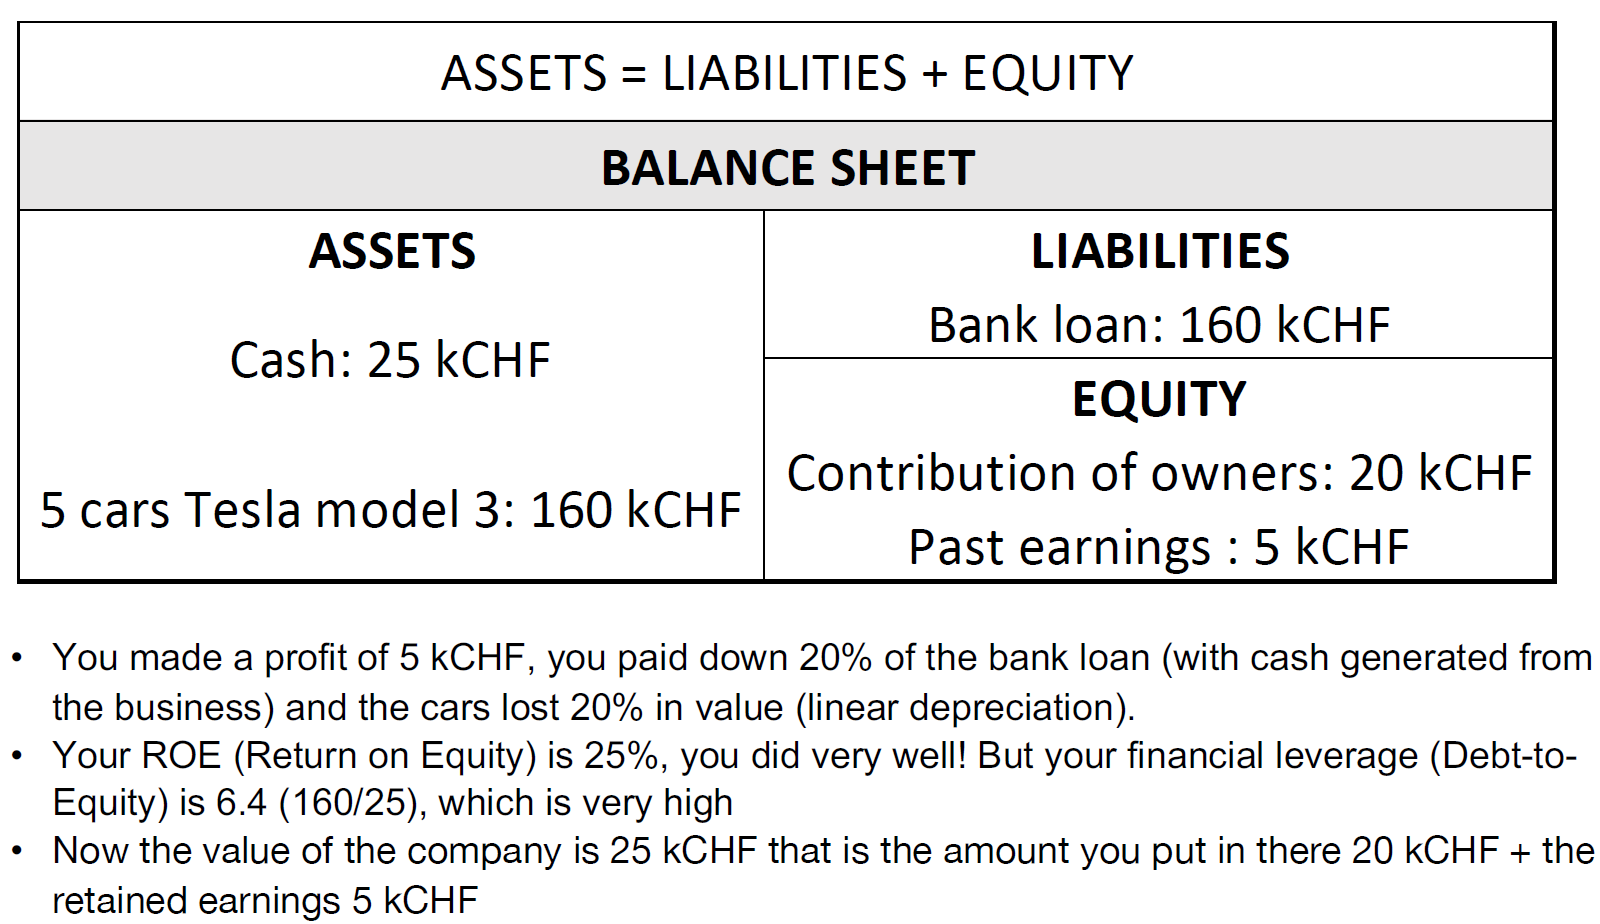
\includegraphics[width=0.5\textwidth]{Pictures/Taxi_example.png}
\end{figure}

However, leverage increases your risk proportionally.

\paragraph{Banking}
Before the financial crisis in 2007/2008 Banks had really high leverage.
It can lead to a domino effect: if one big bank goes bank rupt, others may
suffer as well resulting in the economy to collaps.

\subsection{P \& L - Profit and Loss}

\paragraph{Income Statement}
A Profit and Loss statement, or also called Income statement, summarizes the
revenues, costs and expenses incurred during a specified period, usually a fiscal
quarter or year. It provides information about a company's ability or inability
to generate profit by increasing revenue, reducing costs or both.

\paragraph{Different Components of P \& L}
\begin{itemize}
    \item \underline{Revenues (sales)} = income per hour * operating hours per
        year * occupancy rate * fleet size
    \item \underline{Costs of goods sold} = cost of the material and labor directly
        used to run the business. COGS = operating hours per year * fleet size *
        (costs per hour for the driver + operating costs * occupancy rate)
    \item \underline{Gross Margin} = Revenue - COGS
    \item \underline{OPEX} = Operating Expenses (the remaining costs that are not 
        included in COGS)
    \item \underline{EBIT} = Earnings Before Interest and Taxes (Operating Profit)
        = Gross Margin - OPEX
    \item \underline{EBITDA} = Earnings Before Interest, Taxes, Depreciation and
        Amortization = EBIT + D\&A
    \item \underline{EBT} = Earnings Before Taxes = EBIT - Interest paid
    \item \underline{Net Profit} = EBIT - Interest paid - taxes
\end{itemize}

A company is a 'process'.

\paragraph{Relative valuation and the use of multiples}
In relative valuation, the value of an asset is deduced from the market value
of a set of similar assets. To do relative valuation we need to identify comparable
assets and obtain their market value and standardize these market values, because
absolute prices cannot be compared. This process of standardization creates
price multiples.

\paragraph{Valuation multiples}
\begin{itemize}
    \item \underline{P/E ratio}: Calculate a company's share price (Equity)
        from its earnings (net profit).
    \item \underline{EV/EBITDA ratio}: Calculate a company's Enterprise Value
        from its EBITDA.
    \item \underline{EV/EBIT ratio}: Calculate a company's Enterprise value
        from its EBIT.
\end{itemize}

\begin{figure}[h]
    \centering
    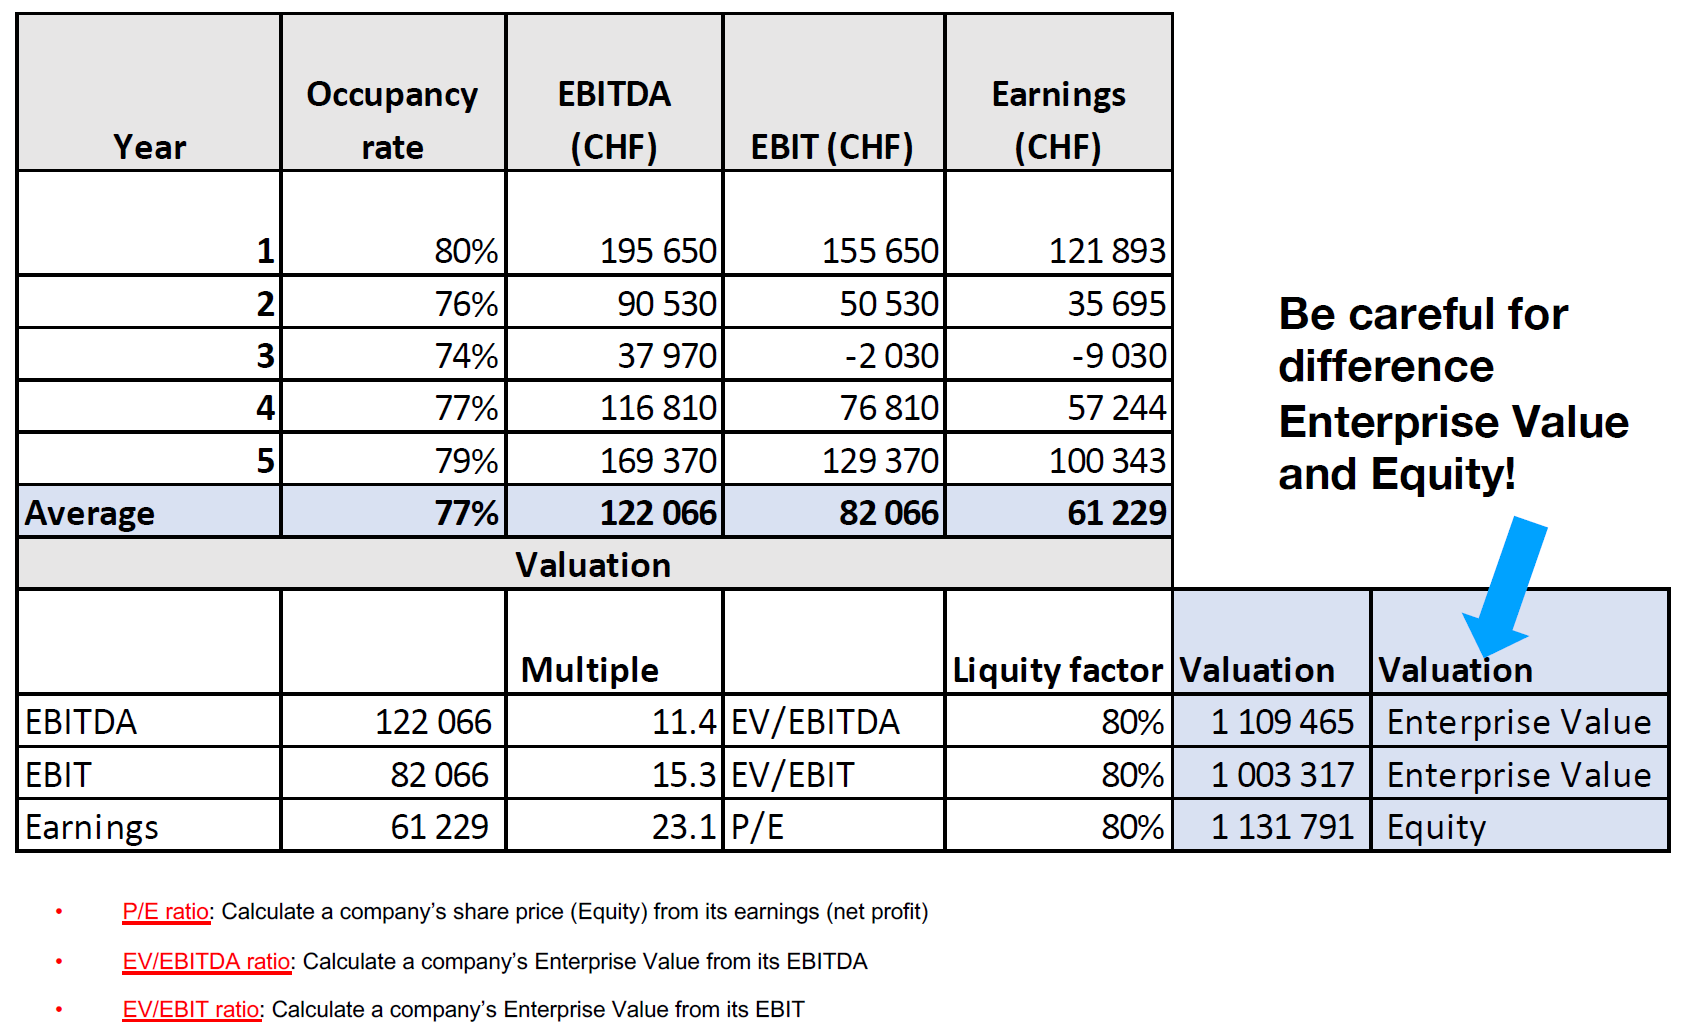
\includegraphics[width=0.7\textwidth]{Pictures/Valuation_taxi.png}
\end{figure}


\subsection{Cash-Flow Statement}
The Cash flow statement consists of three parts: operating activities, investing
activities and financing activities.
\begin{itemize}
    \item Operating Cash flow = Net income + Non cash expenses - increase in Working capital
        \begin{itemize}
            \item Change in Working capital: $\Delta$WC = change in accounts receivable + change in inventory - change in accounts payable
            \item There is a risk of growing too quickly. As a start up when you grow very fast,
                your working capital can also increase very quickly because you have to pay
                your vendors early because they do not trust you and otherwise they will not
                supply, you do not get paid by clients because they have strong negotiation power
                or you have to increase your inventory. As a consequence you can get in serious
                liquidity problems and even go bankrupt because you grow too fast!
        \end{itemize}
    \item Cash Flow from Investing Activities = Purchase/Sale of Long-Term Assets (Capex)
        + Purchase/Sale of other businesses (M\&A) + Purchase/Sale of marketable securities
\item Cash Flow from Financing Activities = Issue/Repurchase equity + Issue/Repurchase Debt
        + Dividend Payments and other Items
\end{itemize}

\begin{figure}[H]
    \centering
    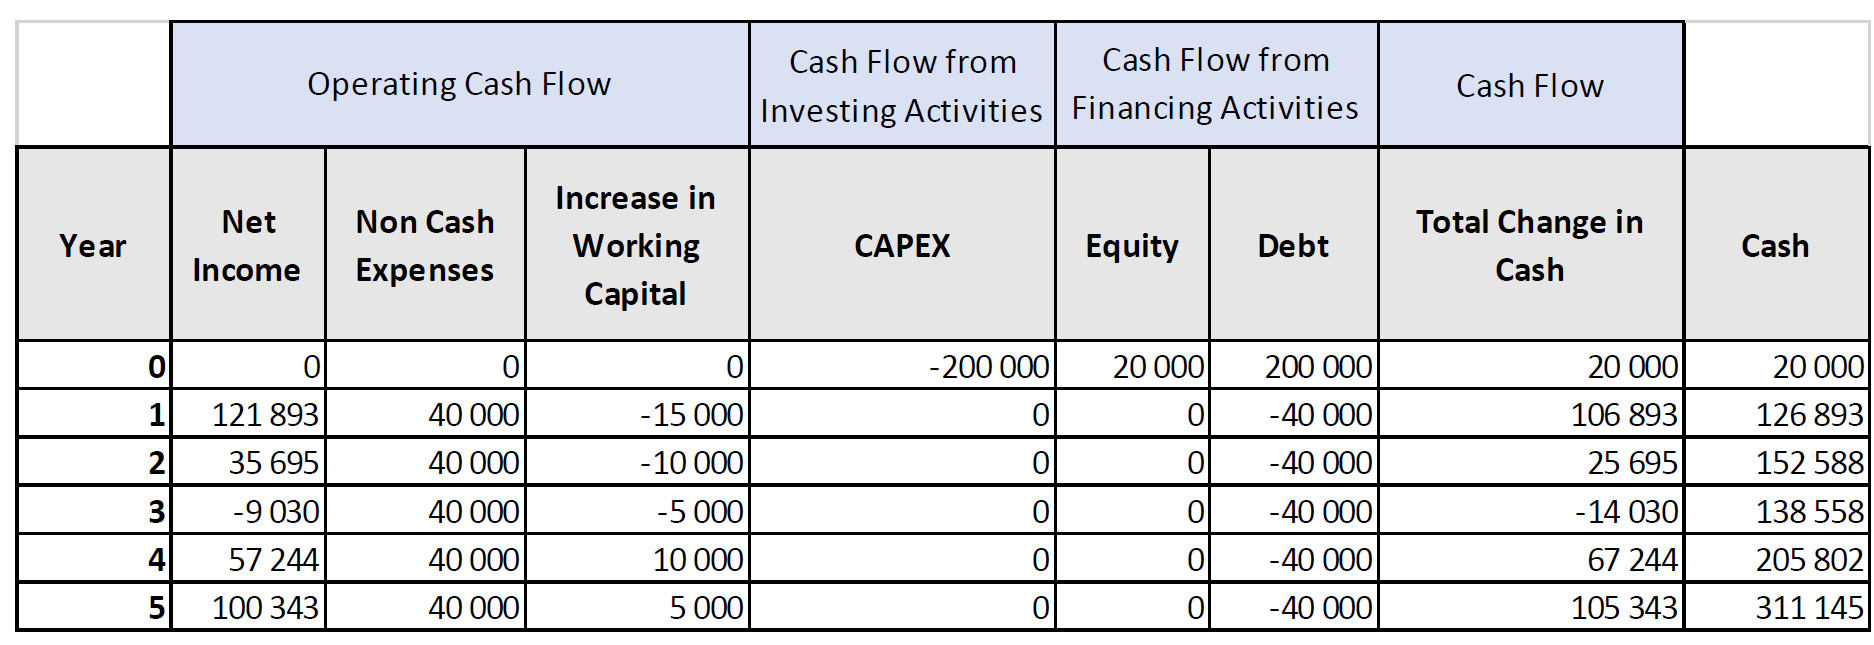
\includegraphics[width=0.8\textwidth]{Pictures/cash_flow_taxi_company.png}
    \caption{Cash flow from Taxi Business}
\end{figure}

\subsection{Company Valuation}

\paragraph{Time value of money}
The Formula for Future value:
\begin{align*}
    FV = PV \times (1+r)^n
\end{align*}
with $FV$ the future value, $PV$ the present value, $n$ the number of periods
and $r$ the rate of return or discount rate or interest rate or growth per period.

\paragraph{Price of a bond}
\begin{align*}
    \text{Bond Price} = \frac{C}{(1+i)} + \frac{C}{(1+i)^2} + \dotsb + \frac{C}{(1+i)^n} + \frac{M}{(1+i)^n}
\end{align*}
Where $C=$ coupon payment, $n=$ number of payments, $i=$ interest rate, or required
yield, $M=$ value at maturity, or par value.

\paragraph{Bonds vs. Stocks}
\begin{itemize}
    \item Bonds:
        \begin{itemize}
            \item Issues of debt
            \item Debt that is made with an investor for cash in exchange for payouts
                of interest.
            \item Typically traded over th ecounter (OTC)
            \item Generally lower risk, lower reward
            \item Since $1929$ have earned around $6\%$ each year
            \item Can be made as corporate, nunicipal, or treasury bonds
        \end{itemize}
    \item Stocks:
        \begin{itemize}
            \item Issues of a stake of ownership in a company
            \item A claim to a company's assets and earnings that often gives
                the investor voting rights and pays dividends
            \item Typically traded through a central exchange (like NYSE)
            \item Generally higher risk, higher reward
            \item Since 1929 have earned around $10\%$ each year
            \item Are issued by companies at a stock exchange as IPOs
        \end{itemize}
\end{itemize}

\paragraph{Discounted Cash Flow Valuation}
Present Value of Discounted Cash Flows:
\begin{align*}
    PV = \frac{CF_1}{(1+r)^1} + \frac{CF_2}{(1+r)^2} + \dotsb + \frac{CF_n}{(1+r)^n}
    = \sum_{i=1}^\infty \frac{CF_i}{(1+r)^i}
    = \sum_{i=1}^\infty \frac{CF_0 [1+g]^i}{(1+r)^i}
    = CF_0 r' \sum_{i=0}^\infty r'^i
    = CF_0 \frac{r'}{1 - r'}
\end{align*}
with $r' = \frac{1+g}{1+r}$, $CF$ the cash flow for a period, $r$ the discount rate and $n$ the number of
periods.
\begin{itemize}
    \item The value of a company can be calculated as the present value of a string
        of cash flows.
    \item There is no maturity so $n = \infty$
    \item Cash flows are not simple coupons like with a bond but must be estimated
    \item $r$ is not the yield of the bond, but is a discount rate that reflects the
        return that the investor expects unter the base case. It depends on the risk
        perception of the investor, higher risk will be high $r$ and vice versa.
\end{itemize}

Valuing a mature business with cash flow growing steadily at $g$:
\begin{align*}
    PV = CF_0 \frac{1+g}{r-g} = \frac{CF_1}{r-g}
    \hspace{10pt} \Rightarrow \hspace{10pt}
    \frac{PV}{CF_1} = \frac{1}{r-g}
    \hspace{10pt} \Rightarrow \hspace{10pt}
    r = \frac{CF_1}{PV} + g
\end{align*}
\begin{itemize}
    \item This is called the dividend discount model or the Gordon-Shapiro formula:
        total return is dividend yield + growth rate
    \item If the company is in a steady state of constant growth, the discounted
        cash flows formula can be written in the form of a multiple
\end{itemize}

\paragraph{Valuing a young company with a $5$ year start-up phase}
\begin{align*}
    PV = \sum_{i=1}^5 \frac{CF_i}{(1+r)^i} + \frac{TV}{(1+r)^5}
    = \sum_{i=1}^5 \frac{CF_i}{(1+r)^i} + \frac{\eckigeklammer{\frac{CF_6}{r' - g}}}{(1+r)^5}
\end{align*}
with $r$ the target rate of return during start-up phase and $r'$ the target
rate of return of mature business.
\begin{itemize}
    \item We discount the estimated cash flows during the start-up phase individually
    \item We calculate the TV (Terminal Value) of the company $5$ years in the future,
        when it has reached a state of maturity growth.
    \item We discount this TV
    \item This is like pricing a bond with estimated coupons and an estimated
        notional value
\end{itemize}

\paragraph{Discount rate}


\begin{itemize}
    \item Cashflows are discounted at a target rate of return, this is set high
        enough to capture business risk and the likelihood that the firm will
        not survive.
    \item Rates decrease as firms move through the life cycle and the chance of
        failure drops.
\end{itemize}

\begin{table}[H]
    \centering
    \begin{tabular}{|c|c|}
        \hline
        Stage of developmend & Typical target rates of return \\ \hline
        Start up & $50\% - 70\%$ \\ \hline
        First stage & $40\% - 60\%$ \\ \hline
        Second stage & $35\% - 50\%$ \\ \hline
        Bridge / IPO & $25\% - 35\%$ \\ \hline
    \end{tabular}
    \caption{Venture capital target rates of return - Stage in Life Cycle}
\end{table}

\begin{table}[H]
    \centering
    \begin{tabular}{|c|c|c|c|c|}
        \hline
        & $3$ years & $5$ years & $10$ years & $20$ years \\ \hline
        Early/Seed VC & $4.90 \%$ & $5.00\%$ & $32.90\%$ & $21.40\%$ \\ \hline
        Balanced VC & $10.80\%$ & $11.90\%$ & $14.40\%$ & $14.70\%$ \\ \hline
        Later Stage VC & $12.40\%$ & $11.10\%$ & $8.50\%$ & $14.50\%$ \\ \hline
        All VC & $8.50\%$ & $8.80\%$ & $16.60\%$ & $16.90\%$ \\ \hline
        NASDAQ & $3.60\%$ & $7.00\%$ & $1.90\%$ & $1.90\%$ \\ \hline
        S\&P & $2.40\%$ & $5.50\%$ & $1.20\%$ & $8.00\%$ \\ \hline
    \end{tabular}
    \caption{Returns earned by Venture Capitalists - 2007}
\end{table}

The actual annual returns earned by VCs at every stage of the process are much
more modest. The high target rates of return that are used for discounting are
not delivered because of the low survival rate.

\paragraph{Summary}
Three ways of valuation:
\begin{itemize}
    \item The balance sheet valuation gives you the company's book value,
        that is its shareholders' equity (capital and reserves), or the
        difference between its assets and liabilities.
    \item This does not take into consideration the fact that a company is
        'a little machine' or 'a process' that generates profit based on people
        (knowledge, learning,\dots), processes (strategy,organisation) and
        stuff (assets,technology,\dots)
    \item If you buy a company, you buy a little profit-making machine (or loss?).
        So it makes sense to use profit generation as a basis in the valuation.
        That is when you do relative valuation based on market calibrated
        multiples and different metrics in the P\&L, e.g. EBITDA, EBIT, net profit,\dots
    \item However, this supposes that the company is in a sort of 'steady state'
        or 'dynamic equilibrium'. For a growth company, earnings will
        increase in the future ans so will its valuation.
    \item For companies that are structured for growth, the discounted cash flow
        approach is needed (however, here a new parameter enters the equation,
        being the discount factor).
\end{itemize}

\subsection{Limits of markets,complex systems and financial bubbles}

\paragraph{Geometric Brownian Motion}
\begin{align*}
    \frac{dP}{P} = \mu \ dt + \sigma \ dW
\end{align*}
with $\frac{dP}{P}$ the percentage return over a time interval $dt$,
$\mu dt$ the drift over a time interval $dt$ and $\sigma dW$ the volatility
over a time interval $dt$. Stocks are supposed to have a constant drift, that
is the return part of the equation, accompanied by random shocks, that is the
risk part of the equaion. The geometric brownian motion random walk implies
that prices follow an exponential track decorated with noise. This is
equivalent to saying that growth rates are constant, that is why market
movements are mostly communicated as percentage changes and not as
dollar changes.

\paragraph{Bubbles}
\begin{itemize}
    \item A bubble starts with a new opportunity or expectation (e.g. a ground-braking
        technoloty)
    \item Smart money flows in, which leads to a first price appreciation
    \item Attracted by the prospect of higher returns, less sophisticated investors follow
    \item Demand goes up as the price increases, and the price goes up as the demand
        increases. This creates a positive feedback mechanism. The market is fully
        driven by behaviour and sentiment and no longer reflects any real
        underlying value.
\end{itemize}

\paragraph{Crash}
\begin{itemize}
    \item At some point, investors start realizing that the process is no
        longer sustainable and the market collapses.
    \item The crash occurs because the market has entered an unstable phase.
        Like a ruler held up vertically on your finger, any small disturbance
        could have triggered the fall.
    \item This mechanism is often not well understood, and a great controversy
        risis about the cause of the crash.
\end{itemize}

\paragraph{Exogenous vs. endogenous processes}
\begin{itemize}
    \item For exogenous processes cause and effect are linearly and logically
        connected. What is important is the trigger, e.g. for the impact of
        an asteroid, the state of the system is irrelevant.
    \item For endogenous processes cause and effect are not linearly connected.
        What is important is the state of the system. Any small event can
        trigger a major incident at some bifurcation points.
\end{itemize}

\paragraph{Complex Systems}
"Complex" does not simply mean "Complicated", is has a very specific meaning:
A complex System consists of a large ensemble of agents, like molecules,
stars, insects, mammals or even human beings. These interact, e.g. they may
repel, attract or imitate each other. Having a large set of interacting
agents is not enough. A system is said to be "complex", when there is
"Emergence", that is when local interactions lead to global cooperation,
in absence of any global orchestration. The whole is different that the sum
of its parts ("More is different" is a quote by Phil Anderson). "More is
different": one star does not make a galaxy; one molecule cannot freeze.
Local interactions lead to global structures.

\paragraph{Emergence}
Coordination in absence of orchestration. Local interactions lead to global
cooperation and self-organization.

\paragraph{Dynamics of human systems}
By imitation and internal organization groups of people may exhibit a global
coorporation. Emergence appears and the mass behaves like a complex system
similarly to a swarm, this is endogenous, there is no master of ceremony at work.
Under such circumstances it is often quite deceptive to follow a cause-and-consequence
reason, what is most important is the state of the system. Any small event can
trigger a major incident.
